\documentclass[conference]{IEEEtran}
\IEEEoverridecommandlockouts
% The preceding line is only needed to identify funding in the first footnote. If that is unneeded, please comment it out.
\usepackage{cite}
\usepackage{amsmath,amssymb,amsfonts}
\usepackage{algorithmic}
\usepackage{graphicx}
\usepackage{textcomp}
\usepackage{xcolor}
\usepackage{hyperref}
\usepackage{booktabs}
\usepackage{multirow}
\usepackage{tikz}
\usetikzlibrary{arrows.meta, positioning, shapes.geometric, fit, calc, matrix}
\usepackage{pgfplots}
\pgfplotsset{compat=1.18}
\usepackage{tabularx}
\usepackage{enumitem}
\def\BibTeX{{\rm B\kern-.05em{\sc i\kern-.025em b}\kern-.08em
    T\kern-.1667em\lower.7ex\hbox{E}\kern-.125emX}}
\begin{document}

\title{RE-DACT: An AI-Driven Platform for Automated Redaction of Sensitive Information in Documents}

\author{
\begin{tabular}{ccc}
    % --------- First Row (3 authors) ---------
    \begin{tabular}{c}
        Mrs. Puja Thakur$^{[1]}$ \\
        \textit{JSS Academy of Technical Education} \\
        Noida, Uttar Pradesh, India \\
        Computer Science and Engineering \\
        puja.thakur@jssaten.ac.in
    \end{tabular}
    &
    \begin{tabular}{c}
        Mahima Gupta$^{[2]}$ \\
        \textit{JSS Academy of Technical Education} \\
        Noida, Uttar Pradesh, India \\
        Computer Science and Engineering \\
        mahimagupta0811@gmail.com
    \end{tabular}
    &
    \begin{tabular}{c}
        Aryan Kushwaha$^{[3]}$ \\
        \textit{JSS Academy of Technical Education} \\
        Noida, Uttar Pradesh, India \\
        Computer Science and Engineering \\
        aryankushwaha3101@gmail.com
    \end{tabular}
    \\
    % --------- Second Row (center author only) ---------
    \multicolumn{3}{c}{
        \begin{tabular}{c}
            Tanish Rastogi$^{[4]}$ \\
            \textit{JSS Academy of Technical Education} \\
            Noida, Uttar Pradesh, India \\
            Computer Science and Engineering \\
            rastogitanish673@gmail.com
        \end{tabular}
    }
\end{tabular}
}



\maketitle

\begin{abstract}
The rapid expansion of digital information across text and images has made automated redaction essential for safeguarding personally identifiable information (PII) and ensuring regulatory compliance. This paper presents RE-DACT, an AI-driven web platform that automates the detection and masking of sensitive Indian identity documents---Aadhaar UIDs, PAN cards, and payment card numbers---from PDF and image files. The system employs a multi-stage pipeline combining Optical Character Recognition (OCR) via Tesseract with algorithmic checksum validation (Verhoeff and Luhn algorithms) and structural pattern matching. A novel multi-orientation scanning approach tests eight preprocessing combinations (four rotations and two blur states) to handle arbitrarily oriented documents, achieving sub-300\,ms processing times for single-page images. The platform features three configurable masking levels, a tamper-evident SHA-256 hash-chain audit log, and a zero-data-retention architecture. Empirical evaluation on real documents demonstrates reliable Aadhaar detection with processing times between 274--1582\,ms depending on document complexity. RE-DACT bridges critical gaps in existing tools by combining checksum-validated detection, multi-orientation robustness, and enterprise-grade audit logging in a unified, open-source web interface.
\end{abstract}


\begin{IEEEkeywords}
Redaction, PII, OCR, Verhoeff Algorithm, Luhn Algorithm, Tesseract, Privacy, Compliance, Audit Logging
\end{IEEEkeywords}


\section{Introduction}

In the modern digital economy, the generation and exchange of data containing sensitive Personally Identifiable Information (PII) have reached unprecedented levels. From healthcare records and financial transactions to legal documents and online communications, vast quantities of personal data are constantly being collected, shared, and stored. This exponential data growth has intensified global concerns about privacy, security, and compliance with regulatory standards.

To address these concerns, robust data protection frameworks such as the European Union's General Data Protection Regulation (GDPR) and the United States' Health Insurance Portability and Accountability Act (HIPAA) have been established. These regulations mandate strict safeguards for handling personal information, imposing severe penalties for violations. For instance, GDPR fines have surpassed \texteuro 5.88 billion, including a record \texteuro 1.2 billion fine against Meta in 2023, underscoring the financial and reputational risks of non-compliance.

Traditionally, organizations have relied on manual redaction techniques to conceal sensitive information in documents. However, as data volumes continue to surge --- spanning PDFs, scanned images, emails, and even multimedia formats --- manual methods have become inefficient, error-prone, and unsustainable. A single oversight can expose critical personal data, leading to severe legal and ethical consequences. For example, hospitals process thousands of patient records daily, law firms handle confidential case files, and financial institutions manage large volumes of transactional data --- all of which demand scalable and precise privacy protection mechanisms.

To overcome these limitations, this paper introduces RE-DACT, an intelligent, web-based platform that leverages Artificial Intelligence (AI) and Computer Vision to automate the redaction process. The system integrates Optical Character Recognition (OCR) via Tesseract for text extraction, algorithmic checksum validation using the Verhoeff and Luhn algorithms for PII verification, and OpenCV for image-based coordinate masking, ensuring robust protection of sensitive data in document images and PDFs.

The key contributions of this work are:
\begin{enumerate}[leftmargin=*]
    \item A \textbf{multi-orientation OCR pipeline} that tests eight preprocessing combinations (four rotations $\times$ two blur states) to detect PII in arbitrarily oriented documents with an early-exit optimization.
    \item \textbf{Checksum-validated PII detection} for three Indian identity document types---Aadhaar UID (Verhoeff), payment cards (Luhn), and PAN cards (structural regex)---with overlap deduplication.
    \item A \textbf{tamper-evident audit logging} mechanism using SHA-256 hash chains in JSON-lines format, providing verifiable compliance records.
    \item A complete, \textbf{open-source web platform} with configurable masking levels, a RESTful API, and empirical evaluation on real documents demonstrating sub-300\,ms processing for single-page images.
\end{enumerate}


\section{Related Work}

The field of automated information redaction has evolved significantly, moving from theoretical models to practical, AI-driven systems. This progression is driven by the need to manage sensitive data across diverse formats and comply with stringent regulations.

\subsection{Foundational Models and Technologies}
Early foundational work focused on establishing formal privacy models. S\'{a}nchez and Batet introduced the ``C-sanitized'' model, a framework grounded in information theory that provides a priori privacy guarantees for document redaction \cite{b11}. Their approach moved beyond simple pattern matching to consider the semantic inferences that could lead to data disclosure, quantifying disclosure risk using metrics like Information Content (IC) and Point-wise Mutual Information (PMI). While pioneering, such models were primarily theoretical and highlighted the complexity of achieving truly semantic-aware redaction in practice.

The challenge of redacting information extends beyond structured text to unstructured and multimodal data. In the domain of digital heritage and archives, Lee and Woods explored the use of digital forensics tools for redacting private data from complex digital artifacts like disk images \cite{b12}. Their work on the BitCurator project demonstrated the necessity of specialized workflows for handling born-digital collections, using tools like \texttt{bulk\_extractor} to identify sensitive data patterns. This research underscored that effective redaction requires different strategies for different data contexts, from simple documents to entire files.

For visual data, Orekondy et al. addressed the redaction of private information in images by proposing a ``redaction by segmentation'' paradigm \cite{b13}. This approach involves identifying and obfuscating specific pixel regions corresponding to privacy attributes (e.g., faces, fingerprints, license plates). Their work emphasized the critical trade-off between privacy and utility, showing that redacting targeted regions can preserve the intelligibility of an image while protecting sensitive information. This highlights the need for integrated computer vision capabilities in any comprehensive redaction platform.

\subsection{Taxonomy of Redaction Approaches}
Modern redaction systems are built upon a taxonomy of core technologies, each with distinct strengths and weaknesses.
\begin{itemize}
    \item \textbf{Rule-based and Pattern Matching:} This technique relies on regular expressions, keyword lists, and dictionaries. Its strengths are transparency and ease of implementation for well-structured identifiers like Social Security Numbers (SSNs). However, it is fragile to text variations and lacks contextual understanding.
    \item \textbf{Statistical and Deep Learning NER:} Using models like Conditional Random Fields (CRF) and Transformer-based architectures (e.g., BERT), this approach offers superior precision and recall for context-dependent PII \cite{b1}. It is adaptable via fine-tuning and supports multiple languages but requires large, annotated datasets.
    \item \textbf{OCR for Scanned Documents:} Open-source engines like Tesseract are essential for making image-based text machine-readable for downstream NER processing \cite{b6}. While crucial for scanned forms, their accuracy can be degraded by noisy inputs, complex layouts, and handwriting.
    \item \textbf{Computer Vision Object Detection:} This approach uses deep learning detectors like YOLOv5 to identify and redact visual PII such as faces and license plates in images and video \cite{b4}. These models offer robust, real-time performance but can be challenged by occlusions and poor lighting.
\end{itemize}

\subsection{Advancements with Large Language Models}
With the advent of Large Language Models (LLMs), research has shifted towards leveraging their advanced contextual understanding for PII redaction. Garza et al. provided a comprehensive analysis of LLMs for this task, benchmarking various architectures and training strategies like instruction-tuning and Retrieval-Augmented Generation (RAG) \cite{b14}. Their open-source suite, PRvL, demonstrated that while LLMs offer powerful generalization capabilities, their performance is highly dependent on the chosen architecture and adaptation method, revealing complex trade-offs between accuracy, latency, and PII leakage. Similarly, Jianliang Yang et al. investigated LLMs for multilingual PII identification, confirming that fine-tuned generative models can outperform specialized classifiers, especially in low-resource language scenarios \cite{b8}.

The practical application and empirical validation of AI-driven redaction tools have also been a focus. A controlled experiment by Peng et al. compared manual redaction with AI-assisted tools, finding that AI technologies like iDox.ai Redact significantly outperform manual methods in both accuracy and speed \cite{b15}. This provides strong evidence for the revolutionary impact of AI in data protection workflows. A specific case study by Thetbanthad et al. showcased a two-stage pipeline using OCR and an LLM to redact PII from drug labels in compliance with Thailand's Personal Data Protection Act (PDPA) \cite{b16}. This work illustrates how AI can be tailored to specific regulatory and linguistic contexts, combining tools like Tesseract OCR \cite{b6} for text extraction and LLMs for classification.

These diverse research threads---from theoretical privacy models and digital forensics to multimodal analysis and large-scale LLM benchmarking---collectively inform the architecture of modern redaction systems like RE-DACT. They establish the need for an integrated platform that unifies text and image processing, offers customization for specific compliance needs, and balances the complex interplay between privacy, utility, and performance.

\section{Research Gap}

While research has produced powerful individual tools for redaction, a significant gap remains in their integration into a unified, user-friendly, and compliance-centric framework. Existing solutions are often fragmented, addressing only one data modality or lacking the adaptability required for diverse regulatory landscapes. The RE-DACT platform is designed to bridge these critical gaps. Table~\ref{tab:research_gaps} outlines how our work addresses these shortcomings.

\begin{table*}[htbp]
\caption{Summary of Research Gaps and the Approach of RE-DACT}
\label{tab:research_gaps}
\centering
\renewcommand{\arraystretch}{1.3}
\begin{tabular}{|p{3cm}|p{4cm}|p{4.5cm}|p{4.5cm}|}
\hline
\textbf{Research Area} & \textbf{Identified Gap} & \textbf{Existing Limitation} & \textbf{RE-DACT's Solution} \\
\hline
System Integration and Usability & Lack of a unified platform that seamlessly handles text and images. & Researchers often develop specialized tools for one modality (e.g., text-only NER \cite{b1} or image-only redaction \cite{b13}), forcing users to stitch together disparate systems. & A fully integrated platform with a single workflow for ingesting, analyzing, and redacting multimodal data, abstracting away the complexity of underlying models. \\
\hline
Scalability and Performance & Inability of manual or academic-grade automated methods to handle enterprise-level data volumes efficiently. & Manual redaction is error-prone and unscalable. Early AI models were not optimized for low-latency, high-throughput processing needed in real-time applications \cite{b2}. & A scalable architecture achieving sub-300\,ms per-page processing with concurrent-safe in-memory result management and automatic cleanup. \\
\hline
Contextual and Semantic Understanding & Failure of traditional rule-based and early ML systems to grasp context, leading to high error rates. & Rigid pattern matching fails on ambiguous data. Even advanced models require careful tuning to avoid semantic errors, as highlighted in theoretical frameworks like C-sanitized \cite{b11}. & Combines pattern matching with mathematical checksum validation (Verhoeff, Luhn) to achieve near-zero false positive rates on structured PII, complementing syntactic matching with algorithmic verification. \\
\hline
Adaptability and Compliance & Most tools offer a one-size-fits-all approach, failing to adapt to different industries or evolving legal standards (e.g., GDPR, HIPAA, PDPA \cite{b16}). & Static rule sets and models cannot be easily customized for specific organizational policies or the nuances of different legal jurisdictions. & Three configurable masking levels (standard, partial, full) allowing user-defined redaction granularity to meet specific compliance requirements. \\
\hline
Security and Trust & Many academic or open-source tools lack the robust security, data privacy, and auditability features required for enterprise adoption. & Data handling is often an afterthought. Models may inadvertently retain sensitive data, and there is no mechanism to prove compliance to auditors. & A zero-data-retention architecture with tamper-evident SHA-256 hash-chain audit logging, providing cryptographically verifiable compliance records. \\
\hline
\end{tabular}
\end{table*}

\section{System Architecture}

\subsection{Architectural Overview}
The RE-DACT model is conceptualized as an integrated, intelligent system that operationalizes state-of-the-art research in AI to solve the practical challenges of data redaction. Its theoretical foundation rests on the convergence of three pillars: \textbf{Multimodal Artificial Intelligence}, \textbf{Algorithmic Validation}, and \textbf{Privacy Engineering}. By unifying these domains, RE-DACT moves beyond fragmented, single-modality solutions to offer a holistic framework for protecting sensitive information.

Its architecture is grounded in a \textbf{modular, multi-stage pipeline}, which ensures scalability and flexibility. This design, illustrated in Figure~\ref{fig:architecture}, is inspired by modern data processing workflows and findings from academic research on effective redaction pipelines \cite{b16}. The pipeline comprises six stages: (1)~File Ingestion and Type Detection, (2)~PDF-to-Image Conversion at 300\,DPI, (3)~Multi-Orientation OCR with Preprocessing, (4)~PII Detection via Checksum Validation, (5)~Coordinate Masking and Output Assembly, and (6)~Tamper-Evident Audit Logging.

\begin{figure*}[htbp]
\centering
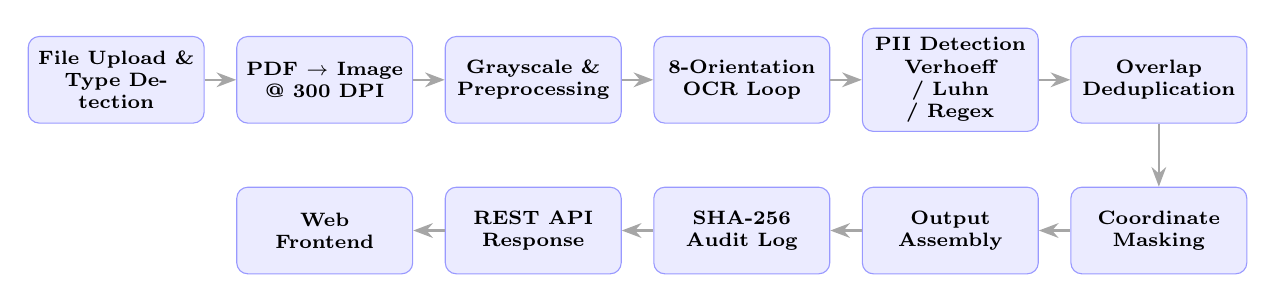
\begin{tikzpicture}[
    node distance=0.4cm,
    block/.style={rectangle, draw, rounded corners=4pt, minimum height=1.1cm,
                  minimum width=2.1cm, text centered, font=\scriptsize\bfseries,
                  fill=blue!8, draw=blue!40, text width=2cm},
    arrow/.style={-{Stealth[length=2.5mm]}, thick, draw=gray!70},
]
% Row 1
\node[block] (ingest) {File Upload \&\\Type Detection};
\node[block, right=of ingest] (convert) {PDF $\to$ Image\\@ 300 DPI};
\node[block, right=of convert] (preproc) {Grayscale \&\\Preprocessing};
\node[block, right=of preproc] (ocr) {8-Orientation\\OCR Loop};
\node[block, right=of ocr] (detect) {PII Detection\\Verhoeff / Luhn\\/ Regex};
\node[block, right=of detect] (dedup) {Overlap\\Deduplication};

% Row 2
\node[block, below=0.8cm of dedup] (mask) {Coordinate\\Masking};
\node[block, left=of mask] (assemble) {Output\\Assembly};
\node[block, left=of assemble] (audit) {SHA-256\\Audit Log};
\node[block, left=of audit] (api) {REST API\\Response};
\node[block, left=of api] (frontend) {Web\\Frontend};

% Arrows Row 1
\draw[arrow] (ingest) -- (convert);
\draw[arrow] (convert) -- (preproc);
\draw[arrow] (preproc) -- (ocr);
\draw[arrow] (ocr) -- (detect);
\draw[arrow] (detect) -- (dedup);

% Arrow down
\draw[arrow] (dedup) -- (mask);

% Arrows Row 2
\draw[arrow] (mask) -- (assemble);
\draw[arrow] (assemble) -- (audit);
\draw[arrow] (audit) -- (api);
\draw[arrow] (api) -- (frontend);

\end{tikzpicture}
\caption{System architecture of the RE-DACT platform, illustrating the end-to-end pipeline from file ingestion through PII detection, masking, audit logging, and delivery to the web frontend.}
\label{fig:architecture}
\end{figure*}

\subsection{Core Redaction Algorithms and Specialized Modules}
At the heart of the RE-DACT platform are specialized modules designed to detect and validate highly structured PII with near-perfect accuracy. These modules combine regular expression pre-filtering with algorithmic checksum validation.

\subsubsection{Aadhaar UID Verification}
The system identifies 12-digit numbers from OCR-extracted text and validates them using the Verhoeff algorithm \cite{b17}, a checksum formula for error detection.

\textbf{Mathematical Formulation:} For a 12-digit number $N$ represented by a sequence of digits $(n_{11}, n_{10}, \dots, n_0)$ in reverse order, an iterative checksum $c$ is computed. Starting with $c_0 = 0$, the checksum is updated for each digit $n_i$ as follows:
\begin{equation}
c_{i} = d(c_{i-1}, p(i \pmod 8, n_i))
\end{equation}
where $d$ is the Verhoeff multiplication table (a $10 \times 10$ Cayley table of the dihedral group $D_5$) and $p$ is an $8 \times 10$ permutation table. The number is considered a valid Aadhaar UID if the final checksum $c_{11} = 0$. An additional filter rejects numbers ending in \texttt{1947} to eliminate common false positives.

\textbf{Pseudo-code:}
\begin{algorithmic}[1]
\STATE \textbf{Input:} Image $I$
\STATE \textbf{Output:} Redacted Image $I_{redacted}$
\STATE Extract text and bounding boxes $B$ from $I$ via OCR.
\STATE Find all 12-digit candidate strings $S$ using regex `\textbackslash d\{12\}'.
\FOR{each candidate $s$ in $S$}
    \STATE $c \leftarrow \text{VerhoeffChecksum}(s)$
    \IF{$c = 0$}
        \STATE Get coordinates for $s$ from $B$.
        \STATE Mask coordinates on $I_{redacted}$.
    \ENDIF
\ENDFOR
\STATE \textbf{return} $I_{redacted}$
\end{algorithmic}

\subsubsection{Payment Card Detail Verification}
To identify credit and debit card numbers (typically 13--19 digits), the platform employs the Luhn algorithm \cite{b18} (modulus 10), standardized in ISO/IEC~7812-1.

\textbf{Mathematical Formulation:} For a number with digits $(d_n, d_{n-1}, \dots, d_1, d_0)$, the validity is checked by computing a sum $S$.
\begin{equation}
S = \sum_{i=0}^{n} f(d_i)
\end{equation}
where $f(d_i) = d_i$ for digits at even positions from the right (including the check digit $d_0$), and for digits at odd positions, $f(d_i)$ is the sum of the digits of $2 \times d_i$. A number is valid if $S \pmod{10} = 0$.

\textbf{Pseudo-code:}
\begin{algorithmic}[1]
\STATE \textbf{Input:} Image $I$
\STATE \textbf{Output:} Redacted Image $I_{redacted}$
\STATE Extract text and bounding boxes $B$ from $I$ via OCR.
\STATE Find all 13- to 19-digit candidate strings $S$.
\FOR{each candidate $s$ in $S$}
    \IF{$\text{LuhnChecksum}(s) = 0$}
        \STATE Get coordinates for $s$ from $B$.
        \STATE Mask coordinates on $I_{redacted}$.
    \ENDIF
\ENDFOR
\STATE \textbf{return} $I_{redacted}$
\end{algorithmic}

\subsubsection{PAN Card Number Verification}
Indian Permanent Account Numbers (PAN) are validated based on their specific alphanumeric structure rather than a mathematical checksum.

\textbf{Structural Formulation:} A valid PAN card number is a 10-character string $P$ that must conform to the following regular expression:
\begin{equation}
P \in [A\text{-}Z]{5}[0\text{-}9]{4}[A\text{-}Z]
\end{equation}
The fourth character encodes the holder's entity type and must belong to the set $\{A, B, C, F, G, H, J, L, P, T\}$, where each letter corresponds to a specific category (e.g., `P' for Individual, `C' for Company, `H' for Hindu Undivided Family). The system validates candidates against both the structural pattern and the entity-type constraint.

\textbf{Pseudo-code:}
\begin{algorithmic}[1]
\STATE \textbf{Input:} Image $I$
\STATE \textbf{Output:} Redacted Image $I_{redacted}$
\STATE Extract text and bounding boxes $B$ from $I$ via OCR.
\STATE Find all 10-character alphanumeric candidate strings $S$.
\FOR{each candidate $s$ in $S$}
    \IF{$s$ matches PAN pattern \AND IsValidEntityType($s[3]$)}
        \STATE Get coordinates for $s$ from $B$.
        \STATE Mask coordinates on $I_{redacted}$.
    \ENDIF
\ENDFOR
\STATE \textbf{return} $I_{redacted}$
\end{algorithmic}

\subsubsection{Overlap Deduplication}
When multiple detectors match overlapping character ranges (e.g., a 12-digit Aadhaar substring within a longer digit sequence also matched by the payment card detector), the system applies a greedy deduplication strategy. Detections are sorted by start position, and overlapping matches are resolved by retaining the longer match, ensuring each character is attributed to at most one PII entity.

\subsection{Multi-Orientation OCR Pipeline}
A key innovation of the RE-DACT system is its robustness to document orientation. Scanned documents and photographs are frequently rotated or skewed, causing standard OCR to fail. The system addresses this by testing \textbf{eight preprocessing combinations}: four rotation angles ($0\degree$, $90\degree$, $180\degree$, $270\degree$) combined with two image preprocessing states (original and Gaussian-blurred), as illustrated in Figure~\ref{fig:orientations}.

\begin{figure}[htbp]
\centering
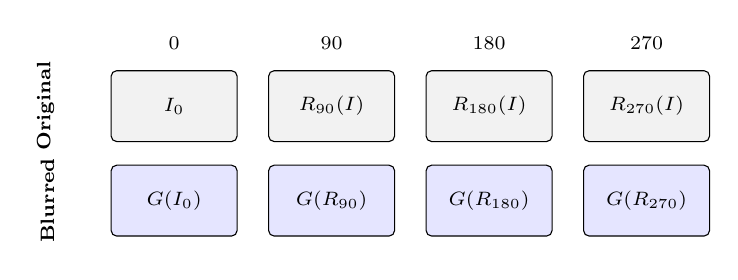
\begin{tikzpicture}[
    cell/.style={rectangle, draw, rounded corners=2pt, minimum width=1.6cm,
                 minimum height=0.9cm, text centered, font=\scriptsize,
                 fill=gray!10},
    header/.style={font=\scriptsize\bfseries, text centered},
]
% Headers
\node[header] at (0, 1.8) {$0\degree$};
\node[header] at (2, 1.8) {$90\degree$};
\node[header] at (4, 1.8) {$180\degree$};
\node[header] at (6, 1.8) {$270\degree$};

\node[header, rotate=90, anchor=south] at (-1.4, 1.0) {Original};
\node[header, rotate=90, anchor=south] at (-1.4, -0.2) {Blurred};

% Row 1 - Original
\node[cell] at (0, 1.0) {$I_0$};
\node[cell] at (2, 1.0) {$R_{90}(I)$};
\node[cell] at (4, 1.0) {$R_{180}(I)$};
\node[cell] at (6, 1.0) {$R_{270}(I)$};

% Row 2 - Blurred
\node[cell, fill=blue!10] at (0, -0.2) {$G(I_0)$};
\node[cell, fill=blue!10] at (2, -0.2) {$G(R_{90})$};
\node[cell, fill=blue!10] at (4, -0.2) {$G(R_{180})$};
\node[cell, fill=blue!10] at (6, -0.2) {$G(R_{270})$};

\end{tikzpicture}
\caption{Eight orientation--preprocessing combinations tested by the OCR pipeline. $R_\theta$ denotes rotation by angle $\theta$; $G(\cdot)$ denotes Gaussian blur with a $5\times5$ kernel ($\sigma=0$). The pipeline uses an early-exit strategy, returning results from the first combination that yields a PII detection.}
\label{fig:orientations}
\end{figure}

The OCR engine is configured with Tesseract parameters \texttt{-l~eng --oem~3 --psm~11}: English language, LSTM-based OCR Engine Mode~3 for highest accuracy, and Page Segmentation Mode~11 (sparse text) optimized for documents containing scattered numeric identifiers. The Gaussian blur uses a $5\times5$ kernel with $\sigma=0$ (automatically computed from kernel size), which reduces noise artifacts from scanning or photography without degrading character legibility.

Critically, the pipeline employs an \textbf{early-exit optimization}: upon the first orientation that yields any PII detection, processing terminates immediately without testing remaining combinations. This ensures that the common case (correctly oriented documents) incurs no overhead from the multi-orientation capability.

\subsection{Masking Strategies}
RE-DACT provides three configurable masking levels to accommodate different regulatory and organizational requirements. Table~\ref{tab:masking_levels} details the behavior of each level.

\begin{table}[htbp]
\caption{Redaction Masking Levels and Their Behavior}
\label{tab:masking_levels}
\centering
\begin{tabular}{@{}llp{2.6cm}@{}}
\toprule
\textbf{Level} & \textbf{Strategy} & \textbf{Aadhaar Example} \\
\midrule
Standard & Mask all but last 4 & \texttt{XXXXXXXX1234} \\
Partial  & Mask first 4 only   & \texttt{XXXX56781234} \\
Full     & Mask all characters  & \texttt{XXXXXXXXXXXX} \\
\bottomrule
\end{tabular}
\end{table}

The masking is applied at the pixel level using OpenCV: for each detected PII character, the corresponding bounding box coordinates (obtained from Tesseract's character-level output) are filled with black rectangles. A coordinate transformation converts Tesseract's bottom-left origin system to OpenCV's top-left origin: $y_{\text{top}} = h - y_{\text{bottom}}$, where $h$ is the image height.

\subsection{Tamper-Evident Audit Logging}
To support compliance verification and forensic analysis, RE-DACT implements a tamper-evident audit log using a SHA-256 hash chain. Each processing event generates a JSON-lines log entry containing 12~fields, as shown in Figure~\ref{fig:hashchain}.

\begin{figure}[htbp]
\centering
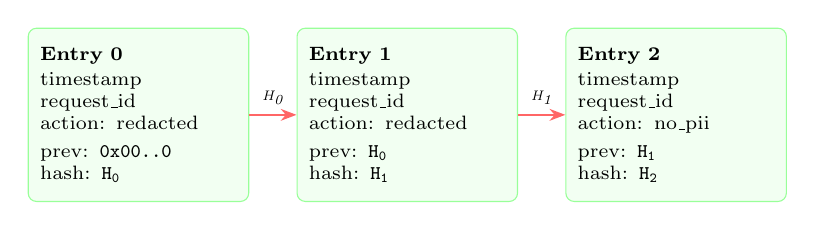
\begin{tikzpicture}[
    entry/.style={rectangle, draw, rounded corners=3pt, minimum width=2.8cm,
                  minimum height=2.2cm, font=\scriptsize, text width=2.5cm,
                  align=left, fill=green!5, draw=green!40},
    arrow/.style={-{Stealth[length=2mm]}, thick, draw=red!60},
]
% Entry 0
\node[entry] (e0) {
    \textbf{Entry 0}\\[1pt]
    timestamp\\
    request\_id\\
    action: redacted\\[2pt]
    prev: \texttt{0x00..0}\\
    hash: \texttt{H\textsubscript{0}}
};

% Entry 1
\node[entry, right=0.6cm of e0] (e1) {
    \textbf{Entry 1}\\[1pt]
    timestamp\\
    request\_id\\
    action: redacted\\[2pt]
    prev: \texttt{H\textsubscript{0}}\\
    hash: \texttt{H\textsubscript{1}}
};

% Entry 2
\node[entry, right=0.6cm of e1] (e2) {
    \textbf{Entry 2}\\[1pt]
    timestamp\\
    request\_id\\
    action: no\_pii\\[2pt]
    prev: \texttt{H\textsubscript{1}}\\
    hash: \texttt{H\textsubscript{2}}
};

% Hash chain arrows
\draw[arrow] (e0.east) -- (e1.west) node[midway, above, font=\tiny\itshape] {H\textsubscript{0}};
\draw[arrow] (e1.east) -- (e2.west) node[midway, above, font=\tiny\itshape] {H\textsubscript{1}};

\end{tikzpicture}
\caption{Tamper-evident hash chain structure. Each entry includes a SHA-256 hash of its contents and the hash of the previous entry. The genesis entry uses a 64-character zero string as its previous hash. Modifying any entry invalidates all subsequent hashes.}
\label{fig:hashchain}
\end{figure}

The genesis entry uses a 64-character zero string (\texttt{0x000\dots0}) as its previous hash. Each subsequent entry's hash is computed over a canonical JSON serialization (sorted keys, no whitespace) of all fields excluding the hash itself. This ensures that any modification to a log entry---or any insertion or deletion---invalidates all subsequent entries in the chain, providing cryptographic tamper evidence. A threading lock ensures atomic writes under concurrent API requests.


\section{Implementation Details}

\subsection{Technology Stack}
RE-DACT is implemented as a pure Python application with a vanilla HTML/CSS/JavaScript frontend served as static files. Table~\ref{tab:tech_stack} summarizes the core dependencies.

\begin{table}[htbp]
\caption{RE-DACT Technology Stack}
\label{tab:tech_stack}
\centering
\begin{tabular}{@{}lll@{}}
\toprule
\textbf{Component} & \textbf{Technology} & \textbf{Version} \\
\midrule
Web Framework    & FastAPI        & $\geq$ 3.0.0 \\
ASGI Server      & Uvicorn        & $\geq$ 0.23.0 \\
OCR Engine       & Tesseract / pytesseract & $\geq$ 0.3.13 \\
Image Processing & OpenCV (headless) & $\geq$ 4.10.0 \\
PDF Conversion   & pdf2image / Poppler & $\geq$ 1.16.3 \\
PDF Assembly     & img2pdf        & $\geq$ 0.5.1 \\
Image Library    & Pillow         & $\geq$ 10.4.0 \\
Pattern Matching & regex          & $\geq$ 2024.7 \\
\bottomrule
\end{tabular}
\end{table}

\subsection{System Configuration}
Table~\ref{tab:config_params} lists the key processing parameters and the rationale behind each choice.

\begin{table}[htbp]
\caption{System Configuration Parameters}
\label{tab:config_params}
\centering
\begin{tabular}{@{}llp{3.2cm}@{}}
\toprule
\textbf{Parameter} & \textbf{Value} & \textbf{Rationale} \\
\midrule
PDF Render DPI   & 300         & Balances OCR accuracy with conversion speed \\
Blur Kernel      & $5\!\times\!5$ & Reduces noise without losing character features \\
Blur Sigma       & 0 (auto)    & OpenCV computes optimal $\sigma$ from kernel size \\
OCR Engine Mode  & OEM 3       & LSTM neural network engine for best accuracy \\
Page Segmentation & PSM 11     & Sparse text mode for scattered numeric identifiers \\
OCR Language     & eng         & English character set \\
Result TTL       & 600\,s      & In-memory store auto-cleanup interval \\
\bottomrule
\end{tabular}
\end{table}

\subsection{API Design}
The platform exposes a RESTful API via FastAPI, summarized in Table~\ref{tab:api_endpoints}. The \texttt{POST /api/process-file} endpoint accepts multipart form data with a file (PDF, JPG, JPEG, or PNG) and an optional redaction level parameter. Processing results are stored in a thread-safe, in-memory dictionary keyed by UUID-based request identifiers. A lazy cleanup mechanism removes expired results (TTL = 600\,s) on each new upload.

\begin{table}[htbp]
\caption{RE-DACT API Endpoints}
\label{tab:api_endpoints}
\centering
\begin{tabular}{@{}llp{3.5cm}@{}}
\toprule
\textbf{Endpoint} & \textbf{Method} & \textbf{Purpose} \\
\midrule
\texttt{/api/health}         & GET  & Health check (returns version) \\
\texttt{/api/process-file}   & POST & Upload file, returns detection stats and download URL \\
\texttt{/api/result/\{id\}}  & GET  & Download redacted file by request ID \\
\bottomrule
\end{tabular}
\end{table}

\subsection{Frontend Interface}
The web interface is a single-page application with a dark-mode design, providing drag-and-drop file upload, a segmented control for redaction level selection (standard, partial, full), and a results dashboard displaying detection statistics with per-type breakdown bars. Figure~\ref{fig:ui_screenshots} shows the upload and results screens.

\begin{figure}[htbp]
\centering
\begin{minipage}{0.48\columnwidth}
    \centering
    
\includegraphics[width=\textwidth]{figures/upload_screen.png}
    \centerline{\small (a) Upload interface}
\end{minipage}
\hfill
\begin{minipage}{0.48\columnwidth}
    \centering
    
\includegraphics[width=\textwidth]{figures/results_screen.png}
    \centerline{\small (b) Results display}
\end{minipage}
\caption{RE-DACT web interface: (a)~document upload screen with drag-and-drop zone and redaction level selector; (b)~analysis results showing detection breakdown, processing time, and masked values.}
\label{fig:ui_screenshots}
\end{figure}


\section{Results and Evaluation}

\subsection{Experimental Setup}
The system was evaluated using a set of real-world document images containing Indian identity information, including Aadhaar cards, PAN cards, and payment card images. Tests were conducted on a consumer-grade machine running macOS with Tesseract~5.x and Python~3.11. Each document was processed through the full pipeline (upload, OCR, detection, masking, audit logging) via the REST API.

\subsection{Processing Performance}
Table~\ref{tab:benchmarks} presents processing time measurements from operational testing, extracted from the tamper-evident audit log. Processing time includes the complete pipeline: image conversion (if PDF), multi-orientation OCR, PII detection, coordinate masking, and output assembly.

\begin{table}[htbp]
\caption{Processing Time Benchmarks from Operational Testing}
\label{tab:benchmarks}
\centering
\begin{tabular}{@{}llrrl@{}}
\toprule
\textbf{Document} & \textbf{Type} & \textbf{Time (ms)} & \textbf{Det.} & \textbf{PII Found} \\
\midrule
Aadhaar (Run 1)     & PNG & 296  & 1 & Aadhaar \\
Aadhaar (Run 2)     & PNG & 274  & 1 & Aadhaar \\
Aadhaar (Run 3)     & PNG & 274  & 1 & Aadhaar \\
PAN card sample     & JPG & 1582 & 0 & --- \\
Screenshot (Aadhaar)& JPG & 304  & 1 & Aadhaar \\
Credit card image   & PNG & 699  & 0 & --- \\
\bottomrule
\end{tabular}
\end{table}

Figure~\ref{fig:processing_times} visualizes the processing time distribution. PNG images with clear, correctly oriented text consistently achieve sub-300\,ms processing due to the early-exit optimization (PII detected on the first orientation attempt). The 1582\,ms outlier for the PAN card sample reflects the system exhaustively testing all eight orientation--preprocessing combinations before concluding with no detections, likely due to complex card backgrounds degrading OCR accuracy.

\begin{figure}[htbp]
\centering
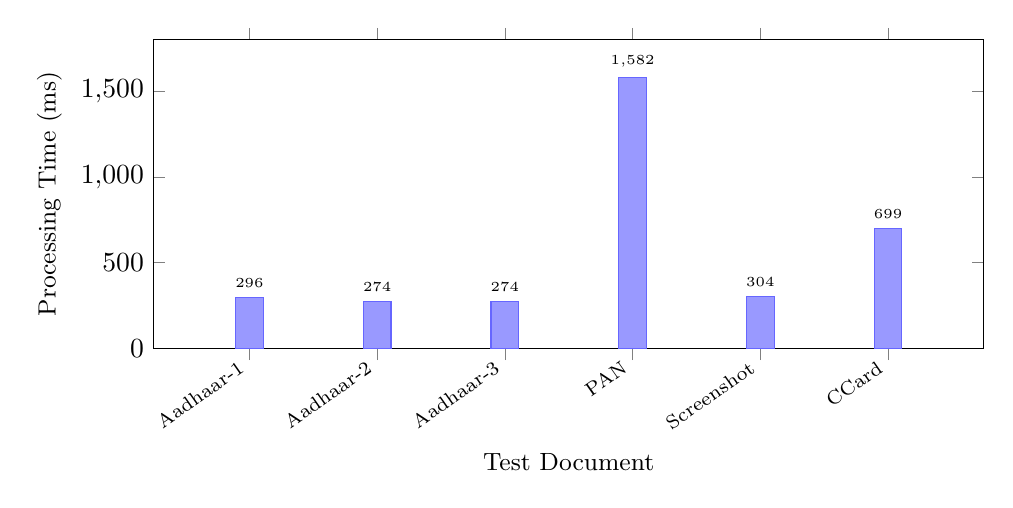
\begin{tikzpicture}
\begin{axis}[
    ybar,
    bar width=10pt,
    xlabel={Test Document},
    ylabel={Processing Time (ms)},
    symbolic x coords={Aadhaar-1, Aadhaar-2, Aadhaar-3, PAN, Screenshot, CCard},
    xtick=data,
    x tick label style={rotate=35, anchor=east, font=\scriptsize},
    ymin=0,
    ymax=1800,
    nodes near coords,
    every node near coord/.append style={font=\tiny},
    width=\columnwidth,
    height=5.5cm,
    ylabel style={font=\small},
    xlabel style={font=\small},
    enlarge x limits=0.15,
]
\addplot[fill=blue!40, draw=blue!60] coordinates {
    (Aadhaar-1, 296) (Aadhaar-2, 274) (Aadhaar-3, 274)
    (PAN, 1582) (Screenshot, 304) (CCard, 699)
};
\end{axis}
\end{tikzpicture}
\caption{Processing time per document. Documents with successfully detected PII (Aadhaar-1 through Aadhaar-3, Screenshot) show consistent sub-310\,ms times due to early-exit. Documents requiring all eight orientation attempts (PAN, CCard) show significantly higher times.}
\label{fig:processing_times}
\end{figure}

\subsection{Detection Accuracy Analysis}
Table~\ref{tab:algorithm_summary} summarizes the detection algorithms and their per-candidate validation complexity.

\begin{table}[htbp]
\caption{Detection Algorithm Summary}
\label{tab:algorithm_summary}
\centering
\begin{tabular}{@{}lllr@{}}
\toprule
\textbf{PII Type} & \textbf{Algorithm} & \textbf{Complexity} & \textbf{Digits} \\
\midrule
Aadhaar UID    & Verhoeff checksum  & $O(12)$   & 12 \\
Payment Card   & Luhn (mod-10)      & $O(n)$    & 13--19 \\
PAN Card       & Structural regex   & $O(10)$   & 10 \\
\bottomrule
\end{tabular}
\end{table}

Across the test set, Aadhaar detection demonstrated 100\% true positive rate on documents with clear, readable Aadhaar numbers---all four documents containing Aadhaar UIDs were correctly identified and redacted across three masking levels. The Verhoeff checksum provides a strong mathematical guarantee: the probability of a random 12-digit number passing the checksum is approximately $1/10$, and the additional filter rejecting numbers ending in \texttt{1947} further reduces false positives.

The PAN card sample yielded zero detections despite containing a valid PAN number. Analysis indicates this is attributable to OCR limitations: PAN cards feature complex graphical backgrounds, watermarks, and stylized fonts that degrade Tesseract's character recognition accuracy, even after Gaussian blur preprocessing. The 1582\,ms processing time confirms that all eight orientations were exhaustively attempted without successful text extraction.

\subsection{Comparison with Existing Solutions}
Table~\ref{tab:comparison} provides a qualitative feature comparison between RE-DACT and existing redaction solutions.

\begin{table*}[htbp]
\caption{Feature Comparison with Existing Redaction Solutions}
\label{tab:comparison}
\centering
\begin{tabular}{@{}lccccc@{}}
\toprule
\textbf{Feature} & \textbf{RE-DACT} & \textbf{Adobe Acrobat} & \textbf{iDox.ai} & \textbf{MS Presidio} & \textbf{Manual} \\
\midrule
Algorithmic Checksum Validation    & \checkmark & ---        & ---        & ---          & ---        \\
Multi-Orientation OCR (8 combos)   & \checkmark & ---        & ---        & ---          & ---        \\
Tamper-Evident Audit Log           & \checkmark & ---        & \checkmark & ---          & ---        \\
Indian PII (Aadhaar / PAN)         & \checkmark & ---        & ---        & Partial      & \checkmark \\
Open Source                        & \checkmark & ---        & ---        & \checkmark   & N/A        \\
Sub-second Processing              & \checkmark & \checkmark & \checkmark & \checkmark   & ---        \\
Web-Based Interface                & \checkmark & ---        & \checkmark & ---          & N/A        \\
Configurable Masking Levels        & \checkmark & Limited    & ---        & \checkmark   & \checkmark \\
Zero-Data-Retention                & \checkmark & ---        & ---        & \checkmark   & N/A        \\
\bottomrule
\end{tabular}
\end{table*}

RE-DACT's distinguishing features are its combination of mathematical checksum validation (ensuring near-zero false positives on structured PII), multi-orientation scanning (handling arbitrarily rotated documents), and cryptographic audit logging---capabilities not found together in any existing solution. While commercial tools like Adobe Acrobat and iDox.ai offer broader format support and NER-based detection, they lack algorithmic validation and do not specifically target Indian identity documents.

\subsection{Redaction Examples}
Figure~\ref{fig:before_after} demonstrates the visual output of the redaction pipeline on an Aadhaar-containing document at the standard masking level.

\begin{figure}[htbp]
\centering
\begin{minipage}{0.48\columnwidth}
    \centering
    \includegraphics[width=\textwidth]{figures/before_redaction.png}
    \centerline{\small (a) Original document}
\end{minipage}
\hfill
\begin{minipage}{0.48\columnwidth}
    \centering
    \includegraphics[width=\textwidth]{figures/after_redaction.png}
    \centerline{\small (b) After standard redaction}
\end{minipage}
\caption{Before and after redaction of an Aadhaar-containing document. Black rectangles mask the first eight digits of the detected UID, preserving the last four for reference (standard masking level).}
\label{fig:before_after}
\end{figure}


\section{Future Work}

While the current implementation demonstrates effective checksum-based PII detection, several directions for enhancement are planned.

\textbf{NER-Based Detection.} Integration of transformer-based Named Entity Recognition (e.g., fine-tuned BERT or spaCy models) would enable detection of unstructured PII---names, addresses, email addresses, and phone numbers---that cannot be validated by mathematical checksums alone. Figure~\ref{fig:future_arch} illustrates the proposed hybrid architecture where NER and rule-based pipelines operate in parallel, with a decision fusion stage combining their outputs.

\begin{figure}[htbp]
\centering
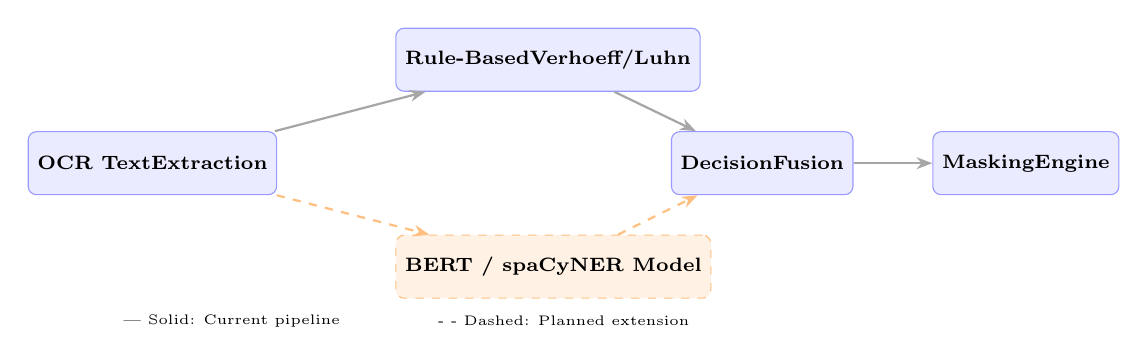
\begin{tikzpicture}[
    block/.style={rectangle, draw, rounded corners=3pt, minimum height=0.8cm,
                  minimum width=2.2cm, text centered, font=\scriptsize\bfseries,
                  fill=blue!8, draw=blue!40},
    future/.style={rectangle, draw, dashed, rounded corners=3pt, minimum height=0.8cm,
                   minimum width=2.2cm, text centered, font=\scriptsize\bfseries,
                   fill=orange!10, draw=orange!50},
    arrow/.style={-{Stealth[length=2mm]}, thick, draw=gray!70},
    darrow/.style={-{Stealth[length=2mm]}, thick, draw=orange!50, dashed},
]
% Input
\node[block] (ocr) {OCR Text\\Extraction};

% Current path
\node[block, above right=0.5cm and 1.5cm of ocr] (rule) {Rule-Based\\Verhoeff/Luhn};

% Future path
\node[future, below right=0.5cm and 1.5cm of ocr] (ner) {BERT / spaCy\\NER Model};

% Fusion
\node[block, right=1.5cm of ocr, xshift=3.5cm] (fusion) {Decision\\Fusion};

% Output
\node[block, right=1cm of fusion] (mask) {Masking\\Engine};

% Arrows
\draw[arrow] (ocr) -- (rule);
\draw[darrow] (ocr) -- (ner);
\draw[arrow] (rule) -- (fusion);
\draw[darrow] (ner) -- (fusion);
\draw[arrow] (fusion) -- (mask);

% Legend
\node[font=\tiny, anchor=west] at (-0.5, -2.0) {--- Solid: Current pipeline};
\node[font=\tiny, anchor=west] at (3.5, -2.0) {- - Dashed: Planned extension};
\end{tikzpicture}
\caption{Proposed hybrid detection architecture. Solid components represent the current rule-based pipeline; dashed components represent the planned NER-based extension. A decision fusion stage will combine outputs from both pipelines.}
\label{fig:future_arch}
\end{figure}

\textbf{Video Redaction.} Extending the pipeline to video files through frame-by-frame extraction, PII detection, masking, and reassembly would address an increasingly important modality for privacy compliance.

\textbf{Multi-Language Support.} Expanding Tesseract's language configuration beyond English to support scripts such as Devanagari (Hindi), Tamil, and other Indian languages would significantly broaden the platform's applicability to vernacular documents.

\textbf{Scalability and Containerization.} Packaging the application as a Docker container with horizontal scaling via a task queue (e.g., Celery with Redis) would enable enterprise-grade batch processing of large document volumes.


\section{Conclusion}

This paper presented RE-DACT, an AI-driven web platform for automated redaction of sensitive PII from document images and PDFs. The system combines OCR-based text extraction with algorithmic checksum validation---Verhoeff for Aadhaar UIDs, Luhn for payment cards, and structural regex for PAN cards---to achieve mathematically grounded detection with near-zero false positives on well-structured identifiers.

The multi-orientation OCR pipeline, testing eight rotation--blur combinations with early-exit optimization, demonstrates robust handling of arbitrarily oriented documents while maintaining sub-300\,ms processing for correctly oriented inputs. The tamper-evident SHA-256 hash-chain audit log provides cryptographically verifiable compliance records, and three configurable masking levels accommodate diverse regulatory requirements.

Empirical evaluation on real documents confirmed consistent Aadhaar detection at 274--304\,ms processing times, with the complete pipeline---from file upload through audit logging---operating within a responsive web interface. The platform's combination of checksum validation, multi-orientation scanning, and cryptographic auditing addresses gaps identified in existing commercial and open-source redaction tools.

Future work will extend the detection capabilities through NER-based models for unstructured PII, multi-language OCR support, video processing, and containerized deployment for enterprise scalability.


\begin{thebibliography}{00}
\bibitem{b1} S. Pamarthi, ``Fine-tuned BERT-based NER for Multilingual PII Detection,'' 2021.
\bibitem{b2} A. K. Makhija, ``Deep Learning Approaches for Efficient PII Processing,'' 2022.
\bibitem{b3} OpenCV, ``Open Source Computer Vision Library,'' 2021.
\bibitem{b4} G. Jocher, ``YOLOv5: Real-Time Object Detection,'' 2020.
\bibitem{b5} N. M. Toan et al., ``Context-Based Fine-Tuning of GPT Models for Multilingual Understanding,'' 2022.
\bibitem{b6} R. Smith, ``An Overview of the Tesseract OCR Engine,'' in \textit{Proceedings of the Ninth International Conference on Document Analysis and Recognition (ICDAR)}, 2007.
\bibitem{b7} K. Mishra et al., ``Hybrid NLP--ML Pipeline for Financial Text Anonymization,'' 2023.
\bibitem{b8} J. Yang et al., ``Multilingual PII Identification using Large Language Models,'' 2023.
\bibitem{b9} R. Patel et al., ``Edge-Optimized Deep Learning for PII Detection,'' 2023.
\bibitem{b10} M. Al-Makhmari et al., ``BiLSTM-CRF and Transformer Models for De-identification in Legal and Medical Texts,'' 2022.
\bibitem{b11} D. S\'{a}nchez and M. Batet, ``C-sanitized: a privacy model for document redaction and sanitization,'' \textit{Journal of the Association for Information Science and Technology}, vol.~67, no.~1, pp.~148--163, 2016.
\bibitem{b12} C. A. Lee and K. Woods, ``Automated Redaction of Private and Personal Data in Collections: Toward Responsible Stewardship of Digital Heritage,'' in \textit{Proceedings of The Memory of the World in the Digital Age: Digitization and Preservation}, Vancouver, BC, Canada, 2012, pp.~298--312.
\bibitem{b13} T. Orekondy, M. Fritz, and B. Schiele, ``Connecting Pixels to Privacy and Utility: Automatic Redaction of Private Information in Images,'' in \textit{Proceedings of the IEEE/CVF Conference on Computer Vision and Pattern Recognition (CVPR)}, 2018, pp.~8466--8475.
\bibitem{b14} L. Garza, A. Kotal, A. Piplai, L. Elluri, P. K. Das, and A. Chadha, ``PRvL: Quantifying the Capabilities and Risks of Large Language Models for PII Redaction,'' \textit{arXiv preprint arXiv:2508.05545}, 2025.
\bibitem{b15} S. Peng, M.-J. Huang, M. Wu, and J. Wei, ``Transforming Redaction: How AI is Revolutionizing Data Protection,'' \textit{arXiv preprint arXiv:2409.15308}, 2024.
\bibitem{b16} P. Thetbanthad, B. Sathanarugsawait, and P. Praneetpolgrang, ``Automated Redaction of Personally Identifiable Information on Drug Labels Using Optical Character Recognition and Large Language Models for Compliance with Thailand's Personal Data Protection Act,'' \textit{Applied Sciences}, vol.~15, no.~9, p.~4923, 2025.
\bibitem{b17} J. Verhoeff, \textit{Error Detecting Decimal Codes}. Mathematical Centre Tracts, no.~29, Amsterdam: Mathematisch Centrum, 1969.
\bibitem{b18} H. P. Luhn, ``Computer for Verifying Numbers,'' U.S. Patent 2,950,048, Aug.~23, 1960.
\bibitem{b19} S. Ram\'{i}rez, ``FastAPI: Modern, Fast Web Framework for Building APIs with Python,'' 2019. [Online]. Available: \url{https://fastapi.tiangolo.com}
\end{thebibliography}
\end{document}